Se ingresan los datos de identificación para iniciar una sesión.
\subsection{Subpaso 1-A: Ingresar credenciales}
\begin{itemize}
	\item Ingrese identificador.
	\item Ingrese contraseña.
	\item Presione el botón \textbf{Entrar}. Este paso puede derivar
		en los errores \textbf{Error E1-A} y \textbf{Error E1-B}.
\end{itemize}
Observación 1: un identificador está compuesto por seis letras seguidas
	de cuatro dígitos.
	
	\begin{figure}[hbtp]
		\centering
		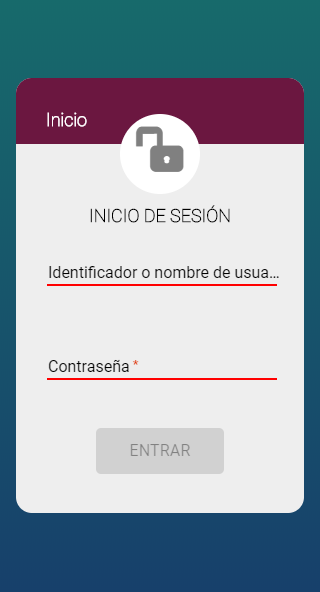
\includegraphics[scale=0.3]{images/InterfazMovil/IUGS00_login.png}
		\caption{Iniciar sesión}
	\end{figure}
	

\subsection{Error E1-A: usuario no registrado}
El identificador que se ingresó no se encuentra registrado en el sistema.
\begin{itemize}
	\item Presionar \textbf{Aceptar} en la ventana emergente 
		\textbf{IUGS-30: usuario no registrado}
\end{itemize}

\subsection{Error E1-B: contraseña equivocada}
La contraseña que ingresó no concuerda con el valor que se tiene almacenado.
\begin{itemize}
	\item Presionar \textbf{Aceptar} en la ventana emergente 
		\textbf{IUGS-31: contraseña equivocada}
\end{itemize}
